\newpage

\section{Simulation study}
In this section, HMMs are trained based on the estimation procedure described in \cref{section:estimation}. The primary purpose of the section is to compare how well different estimation methods converge toward the true parameter values, when data is simulated from an HMM. The advantage of using simulated data is that it entails us knowing the true parameter values. Thus, it becomes possible to directly analyze whether a model has learned the estimates close to the true parameter values, as opposed to relying on general measures of fit, such as AIC and BIC scores, which is necessarily the case when one works with real data. More importantly, simulated data allows us to compare the true state sequences with the estimated. This can be highly informative as it allows the measurement of accuracy in state classification. Simulation will be carried out under various alterations designed to test models' convergence when some of their key assumptions about the data are (partially) unfulfilled\footnote
{Such as the maximum likelihood estimator, which assumes conditional normality. Since it has been shown that e.g. conditional students t-distributions are often a better fit (Bulla, 2011) the assumption is in practice often not fulfilled.
}.

In the following, accuracy of state predictions is defined using recall/sensitivity $\frac{tp}{tp+fn}$, where $tp$ is the number of true positives, and $fn$ is the number of false negative. It measures how large a fraction of all positives that the model is able to detect. When the true state is one, then the positive class will also be one, and the negative class will be all other predictions, when the true state is two the positive class will be two$,\ldots,$ and so on. However, one of the issues with recall is its inability to account for imbalanced data sets. To account for this, Nystrup et al. (2020) suggested using the balanced accuracy score (BAC), which is the average of accuracy in each observed state
\begin{equation}
    BAC = \frac{1}{K} \sum_{k=1}^K \frac{tp_k}{tp_k + fn_k}
\end{equation}
where $tp_k$ is the number of true positives and $fn_k$ is the number of false negatives in state $k$. As a result, when a classifier performs equally well on all states, then BAC reduces to regular accuracy, but if a classifier only performs well by always predicting the dominating class then BAC appropriately drops to the reciprocal of the number of states. So, given data with two classes, then if 99\% of data belongs to the positive class and this is correctly detected, but the remaining 1\% belong to the negative and is incorrectly classified, then that classifier obtains a BAC of 0.50, whereas regular accuracy would be 0.99. Considering the previously mentioned gain/loss asymmetry in financial returns, where losses occur less frequently yet their movements are on average larger than the corresponding movements in gains, BAC behaves exactly as desired.

An inherent problem with comparing several HMMs is the fact that, given the unsupervised nature of the model, it outputs label-less states (predictions). This is, not only the case in this simulation study where thousands of models will be compared, but also the case when backtesting e.g. an HMM based on rolling windows on financial data. For example, consider training two HMMs by MLE on the same data with hidden states a and b. Then differences among their final parameter values and state sequences are entirely attributable to the initialized parameter values (as explained in \cref{section:estimation}, which are random quantities. If the models are initialized in a way where the first model labels state a as 1 and state b as 2, whereas the second model might have the order reversed, thus making comparisons of the two (perhaps equally good) models difficult. There are several ways to circumvent this issue, such as choosing the labels that maximize the accuracy score, however, since this is impossible to do on real data another method is used here. Since a fundamental assumption in this paper is that the primary difference between conditional Gaussian states, is the conditional variance, parameters and state labels are sorted according to variance. Another option could have been sorting according their means, however, when thinking about a "good" and "bad" state it is certainly a possibility to observe a state with a high mean and high variance, which we would still interpret as the "bad" state, therefore making such sorting a poor choice.

The rest of the section is structured as follows: First, the simulation procedure is described. Then we describe how to tune the jump penalty $\lambda$ in the jump model. Once the penalty has been tuned, the models can be trained on simulated data and compared. Initially models are trained on correctly specified conditional distributions, after which we show their performance when conditional distributions are purposely misspecified - a feature that is likely when estimating HMMs on real data.

\subsection{Simulation procedure}

Throughout the section, data is simulated from a 2-state HMM. To make results comparable to those of Nystrup et al. (2020), the same parameters are chosen, thus yielding the Gaussian HMM
\begin{equation*}
    O_t|S_t \sim N(\mu_{st}, \sigma_{st}^2)
\end{equation*}
with parameters
$$
    \mu_{S_t}=
    \begin{cases}
        \mu_1= 0.0123 \\
        \mu_2= -0.0157
    \end{cases}, \quad
    \sigma_{S_t} =
    \begin{cases}
        \sigma_1 = 0.0347 \\
        \sigma_2 = 0.0778
    \end{cases}, \quad
    \mathbf{A} = 
    \begin{bmatrix}
        0.9629 & 0.0371 \\
        0.2101 & 0.7899
    \end{bmatrix}
$$
The model is estimated by Hardy's (2001) using monthly returns, which has been shown to capture many stylized facts of financial times series such as volatility clustering and leptokurtosis. There is a significant overlap between the two states, making it challenging to correctly infer the unobserved state sequence. By assuming instantaneous log-returns follow a Lêvy process, the parameters are transformed from one time scale $t_1$ to another $t_2$ using
\begin{align*}
    \mu_s(t_1) / t_1 &= \mu_s(t_2) / t_2 \\
    \sigma_s(t_1) / \sqrt{\sigma_s(t_1)} &= \sigma_s(t_2) / \sqrt{\sigma_s(t_2)} \\
    \mathbf{A}(t_1)^{1/t_1} &= \mathbf{A}(t_2)^{1/t_2}
\end{align*}

where $\mu(t), \sigma(t)$ and $\mathbf{A}(t)$ are parameters associated with time scale t. Assuming there is twenty trading days in a month, i.e. $t_{monthly}=20$ and $t_{daily}=1$, monthly parameters are transformed into daily
$$
    \mu_{S_t}=
    \begin{cases}
        \mu_1= 0.0615 \times 10^{-2} \\
        \mu_2= -0.0785 \times 10^{-2}
    \end{cases}, \quad
    \sigma_{S_t} =
    \begin{cases}
        \sigma_1 = 0.7759 \times 10^{-2} \\
        \sigma_2 = 1.7400 \times 10^{-2}
    \end{cases}, \quad
    \mathbf{A} = 
    \begin{bmatrix}
        0.9979 & 0.0021 \\
        0.0120 & 0.9880
    \end{bmatrix}
$$

Each series simulated from this model is generated as follows: The first element $s_0$ is drawn from the stationary distribution $\pi$, and each subsequent element is drawn from $q_{t-1}$, i.e. the row of $Q$ corresponding to the last state sojourn. Based on the value of each $s_t$, observations $o_t$ are generated from the conditional distributions. By repeating this procedure, 1000 different series are simulated with sample lengths $H = 250, 500, 1000, 2000$

\subsection{Choosing the jump penalizer}
\label{subsection: jump_penalizer}

\textbf{This section should be expanded to consider different feature sets in the jump estimator - Feature selection is just as important as choosing penalizer.}

Since the MLE model doesn't have any hyperparameters, it can be applied to the simulated data right away. However, that is not the case for the jump model which requires a given value for $\lambda$. As mentioned previously, we are testing the models' ability to correctly identify state sequences, thus we want to maximize BAC with respect to $\lambda$. Since BAC is a random quantity\footnote
{It is a function of the data and the initial state sequence $s_0$, which in the jump estimator is generated by K-means++. Both quantities are random.
},
we define the estimator $\Omega(\lambda)= \mathbb{E}[BAC|\lambda]$, which is maximized with respect to $\lambda$. This can be estimated by 
\begin{equation}
    \hat\Omega(\lambda) = \frac{1}{N} \sum_{i=1}^N BAC_{i, \lambda}^H
\end{equation}
where N is the amount of simulated series, and $BAC_{i, \lambda}^H$ refer to the BAC of the $i$th sequence of sample size H computed using a jump model with penalty $\lambda$.

We proceed, by computing $BAC_{i, \lambda}^H$ on samples of lengths 250, 500, 1000 and 2000. Further, penalties are considered on a grid defined on the logarithmic scale with base 2. Initially the grid was defined on a logarithmic scale with base 10, but evidently this was too course to yield meaningful results. Grid points are equidistantly placed on the closed interval $[2^{-2}, 2^{7}]$. Results are shown in \cref{fig:jump_penalties}. As evident by the figure, the primary difference between simulation lengths is the size of BAC, which is generally increasing with sample size. Once $\lambda$ is below a certain threshold, in this case around $2^5$, BAC isn't too sensitive to the precise level of the penalty. As noted earlier, when $\lambda$ is sufficiently small, BAC converges to the unpenalized case, which is essentially the same as applying a K-means model where the time ordering of observations is irrelevant. For $\lambda$ too large, the jump estimator only identifies the dominating state, and as a result BAC drops to 0.50. 

\begin{figure}[H]
    \centering
    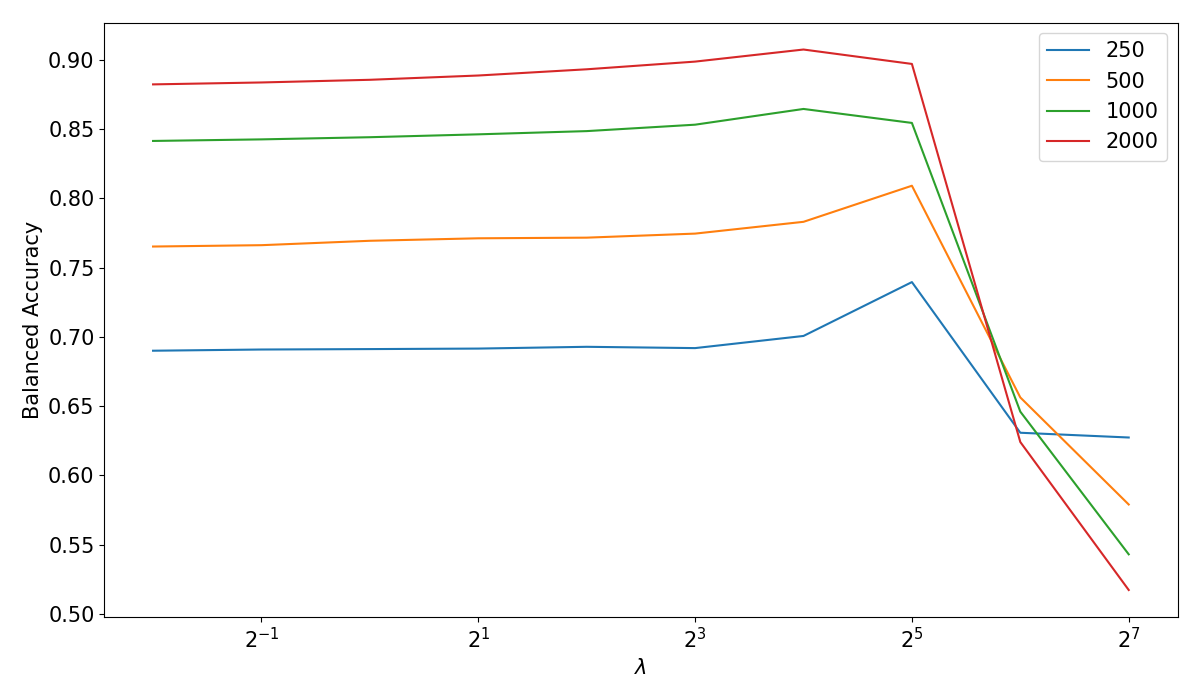
\includegraphics[width=1\textwidth]{analysis/model_convergence/images/jump_penalties.png}
    \caption{Balanced accuracy of jump estimator, as a function of the penalty $\lambda$ using different simulation lengths. All points are based on the estimate $\hat\Omega(\lambda)$ based on 1000 simulated series.}
    \label{fig:jump_penalties}
\end{figure}

From \cref{fig:jump_penalties}, the optimal level of $\lambda$ is roughly equivalent for all simulation lengths, though for $H=250,500$, the optimal penalty is bit higher. As the difference is still quite small, and more importantly, due to the large drop in BAC across all simulation lengths for $\lambda > 2^5$, the optimal penalty is chosen as $\lambda=2^4$ for all simulation lengths. 

\textbf{Consider discussing time-variation in $\lambda$ and how the size of $\lambda$ relates to the size of means in feature matrix.}

\subsection{Simulation study with correctly specified distributions}

\cref{tab:jump_gaussian} and \cref{fig:jump_normal} summarizes the performance of the MLE and Jump estimator for various sample sizes when compared to the true values. As mentioned in the previous section, data is generated from a conditional gaussian HMM, which is also the case for the models trained here. Apart from the HMM parameters, the accuracy in each state as well as BAC is reported. Accuracy for for the true parameters are obtained by running the Viterbi algorithm using an HMM with the true model parameters. This can be seen as the best obtainable performance in state detection and is used to get a sense of where the 'upper bound' on BAC lies when comparing the other models.

\begin{figure}[H] 
    \centering
    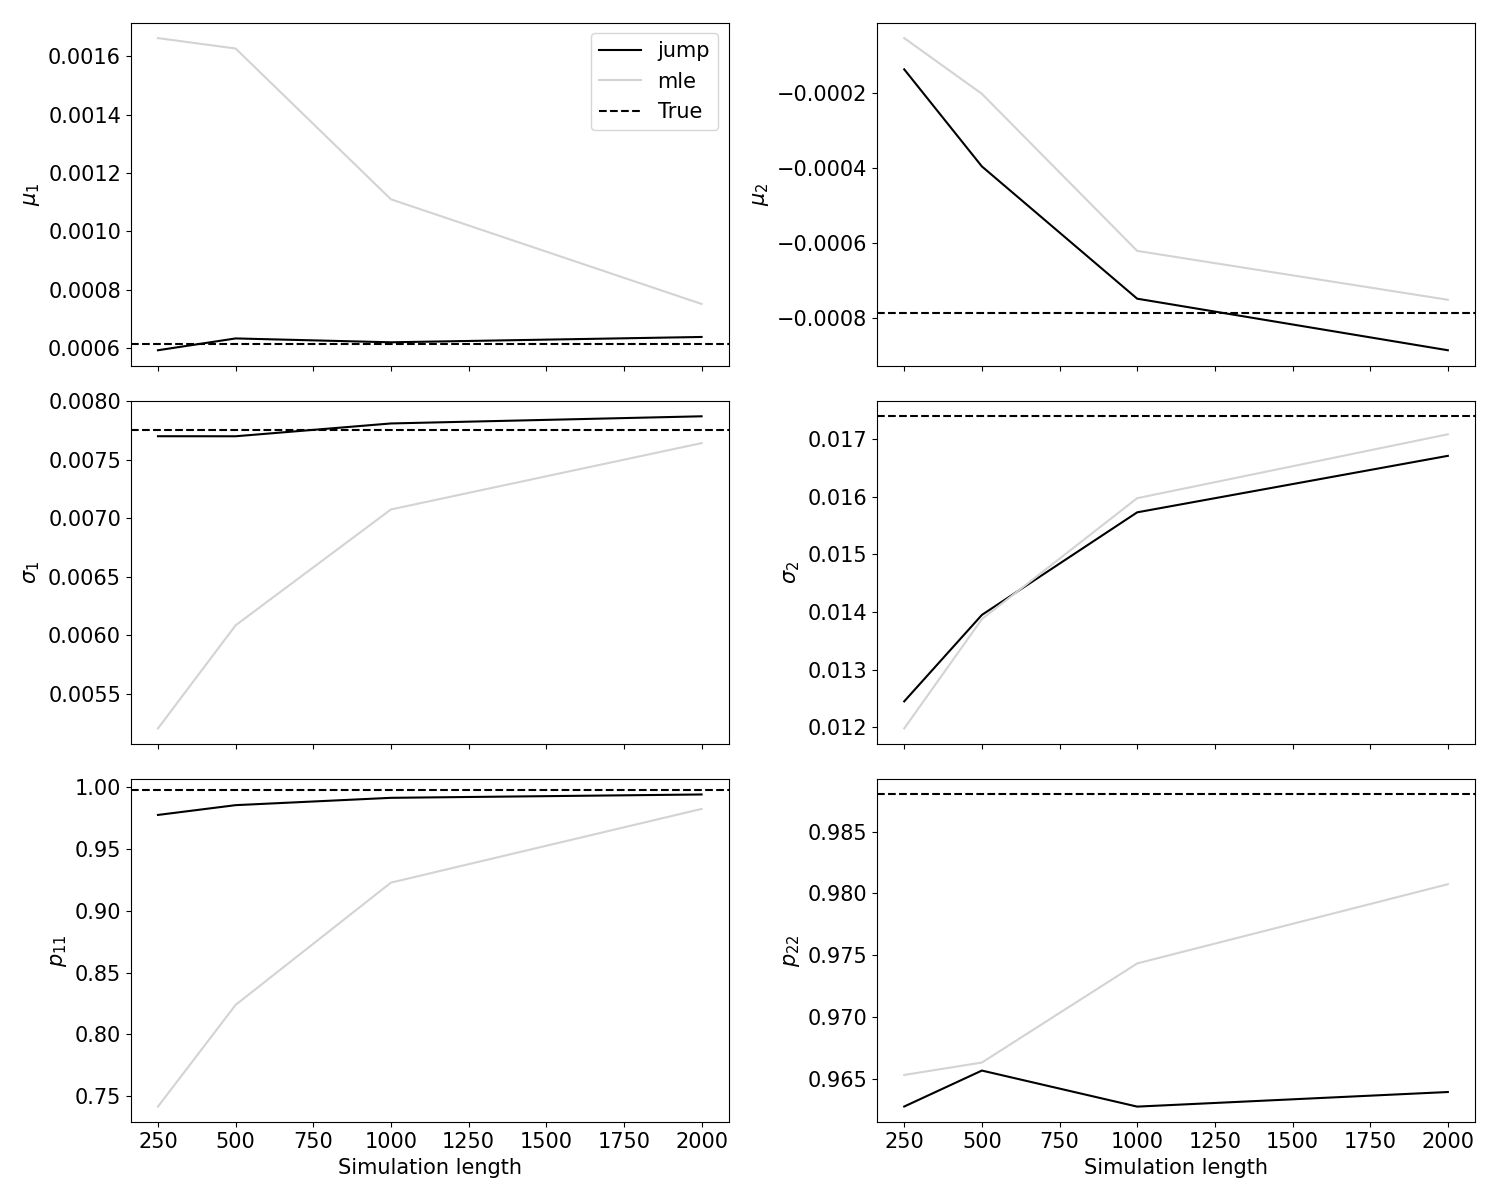
\includegraphics[width=1\textwidth]{analysis/model_convergence/images/simulation_normal.png}
    \caption{Estimates of HMM models' convergence towards true values as a function of simulation length. Results are based on 1000 simulations from conditional gaussian distributions.}
    \label{fig:jump_normal}
\end{figure}

It is clear that that both models converge towards the true values when longer simulation lengths are considered. Curiously, the jump estimator is able to detect the low-variance / high-persistence state quite accurately, even at the shortest simulation lengths. Yet, both models performs poorly on the high-variance / low-persistence state for simulation lengths below 1000. This is most likely explained by the fact that, at low simulation lengths the probability of seeing both states are quite low. For a series of 250 observations the probability of only seeing one state is 51\%, at 500 observations it is 30\%, for 1000 observations it is 10\% and at 2000 observations it is 1\%\footnote
{These probability are calculated using the fact that sojourn times follows a geometric distrubution.
}. 
When only one state is observed, it becomes inherently harder for the estimator to detect that only one state is actually present, when it is designed to fit two.

Previous studies such as Zheng et al. (2019), alleviated this problem by excluding those simulations with only one state present, however as noted by Nystrup et al. (2020) this introduces bias in the transition probabilities. The problem with excluding those simulations, is that when training HMMs on real data, then it possible that only one state will be present at times. This is especially true when one is considering a rolling window. In such cases, it is important that the estimator doesn't break down, which for example, is regularized with the jump penalty in the jump estimator. For most parameters, both models converge toward the true parameters around 1000 and 2000 observations, though convergence speed quickly decreases for sequences longer than that.

In conclusion, the different estimators generally converge towards the true parameter values when the simulation length is increased. However, these results are dependent on the assumption that the underlying distribution of data is known, which is generally unrealistic - especially with financial returns. In the following section we show how the estimators perform when they are purposefully estimated on an unknown distribution, which is not a mixture of gaussian distributions.


\begin{table}[H]
\centering
\caption{Estimates of HMM models' convergence towards true values as a function of simulation length. Results are based on 1000 simulations from conditional gaussian distributions.}
\begin{tabular}{llrrrrrr}
\toprule
     &      &  $\mu_1$ &  $\mu_2$ &  $\sigma_1$ &  $\sigma_2$ &  $q_{11}$ &  $q_{22}$ \\
sample_size & model &          &          &             &             &           &           \\
\midrule
250  & true &   0.0006 &  -0.0008 &      0.0078 &      0.0174 &    0.9979 &    0.9880 \\
     & mle &   0.0017 &  -0.0000 &      0.0052 &      0.0121 &    0.7410 &    0.9658 \\
     & jump &   0.0006 &  -0.0001 &      0.0079 &      0.0113 &    0.9770 &    0.8903 \\
500  & true &   0.0006 &  -0.0008 &      0.0078 &      0.0174 &    0.9979 &    0.9880 \\
     & mle &   0.0015 &  -0.0002 &      0.0060 &      0.0139 &    0.8152 &    0.9719 \\
     & jump &   0.0006 &  -0.0003 &      0.0079 &      0.0130 &    0.9834 &    0.8898 \\
1000 & true &   0.0006 &  -0.0008 &      0.0078 &      0.0174 &    0.9979 &    0.9880 \\
     & mle &   0.0011 &  -0.0006 &      0.0071 &      0.0160 &    0.9208 &    0.9763 \\
     & jump &   0.0006 &  -0.0006 &      0.0080 &      0.0152 &    0.9866 &    0.9420 \\
2000 & true &   0.0006 &  -0.0008 &      0.0078 &      0.0174 &    0.9979 &    0.9880 \\
     & mle &   0.0008 &  -0.0007 &      0.0076 &      0.0171 &    0.9823 &    0.9817 \\
     & jump &   0.0006 &  -0.0007 &      0.0080 &      0.0164 &    0.9951 &    0.9679 \\
\bottomrule
\end{tabular}

\label{tab:jump_gaussian}
\end{table}


\subsection{Simulation study with misspecified distributions}

In this section, the simulation procedure from before is repeated, except for that fact that observations are sampled from conditional student's t distribution instead of gaussian, though means, variances and transition probabilities remain unchanged. The simulated t-distribution has five degrees of freedom. Student's t distribution generally have fatter tails, and have been shown to better resemble financial returns compared to normal distributions (Cont, 2001). As such, the goal of this section is to create a more realistic simulation experiment, in which models are still specified to be conditional gaussian, even though the simulated data is not. When implementing these types of models in a portfolio, it is important to know how it performs in such an environment. The results in this section will thus provide insights into how well each estimator performs in such a scenario, and where they fail.

\cref{fig:jump_t} shows the mean parameter values as a function of simulation length based on 1000 simulations. Compared to \cref{fig:jump_normal}, the estimators performance has generally worsened. Yet, the jump estimator is generally more robust, especially when analyzing the transition probabilities, in which the jump estimator has close to similar performance as before. As mentioned in \cref{subsection: Jump theory}, a large advantage of the jump model is that, during training it does not assume anything about the distributional properties of the data, therefore making it more robust when the data's distribution is unknown.

\begin{figure}[H] 
    \centering
    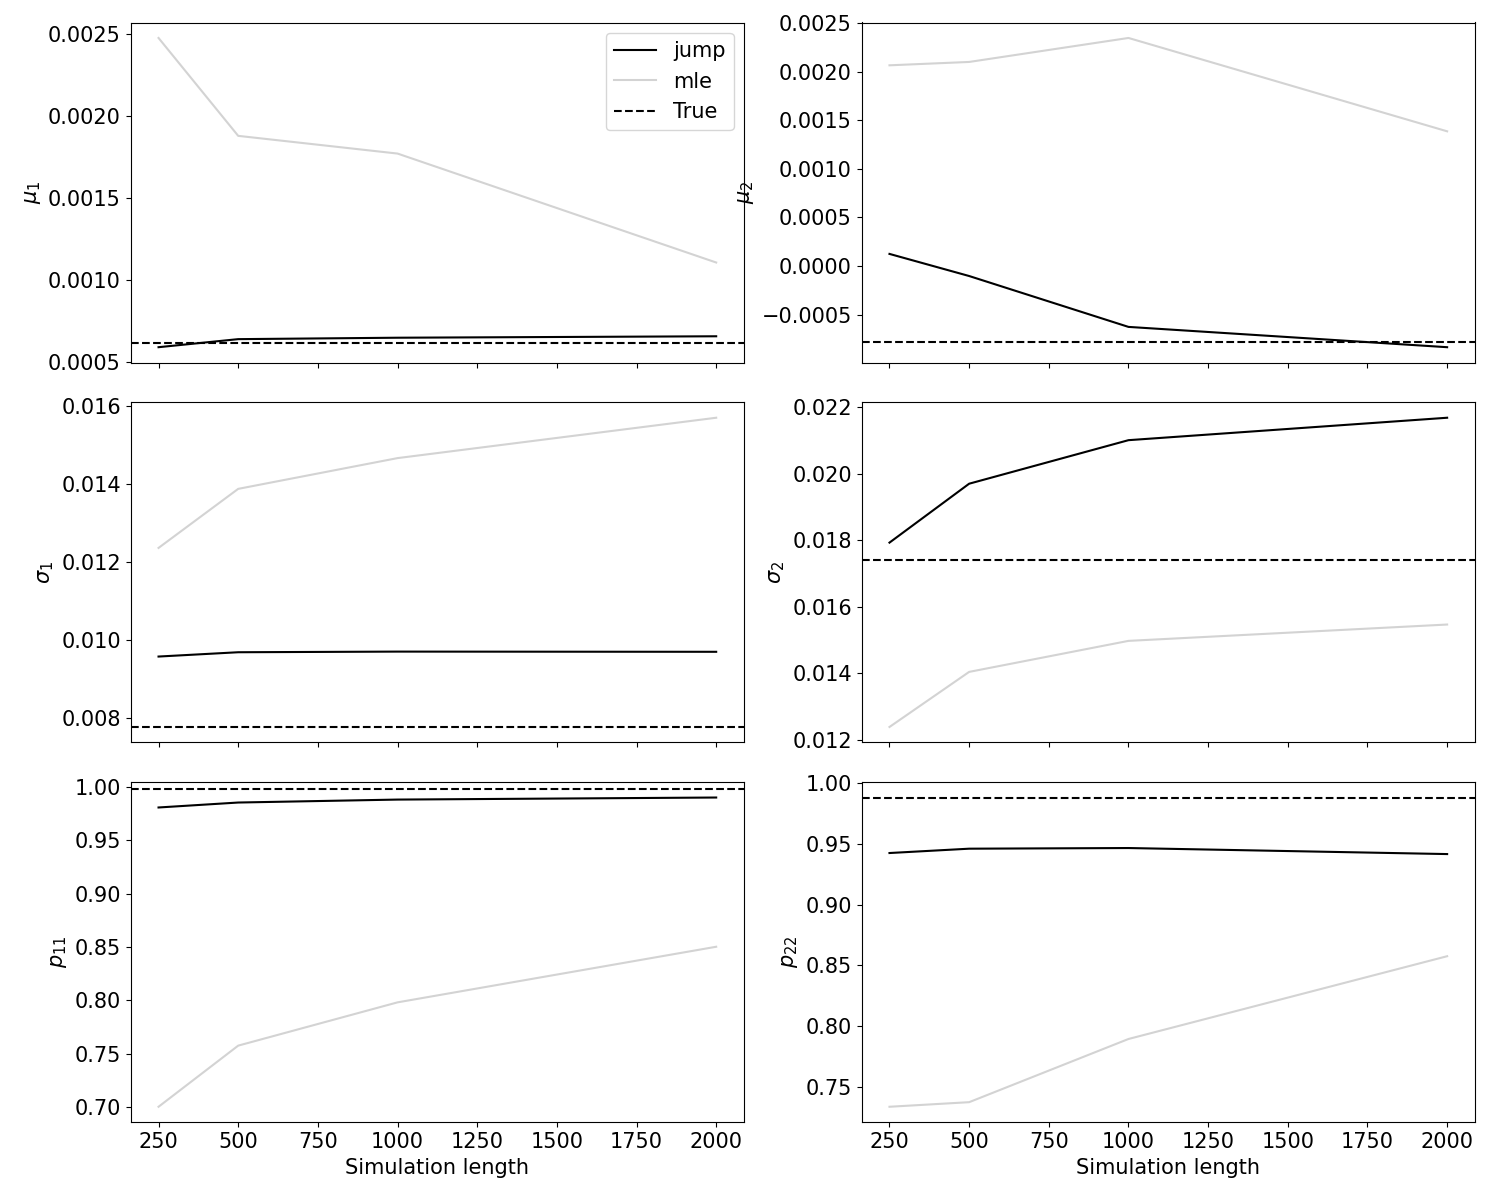
\includegraphics[width=1\textwidth]{analysis/model_convergence/images/simulation_t.png}
    \caption{Estimates of HMM models' convergence towards true values as a function of simulation length. Results are based on 1000 simulations with conditional t distributions with five degrees of freedom.}
    \label{fig:jump_t}
\end{figure}

This is in contrast to the MLE model, which assumes a given conditional distribution for each state during training. From \cref{fig:jump_t} it becomes clear that such an assumption has a sizeable error as the model generally doesn't perform well across the parameters. Most conspicuously, the MLE model has basically broken down in terms of the transition probabilities where it is very far from the true estimates. This would result in states with very low persistence and frequent state switching. Though it does seem to be converging slowly toward the true parameter values, it is much less robust than the jump model. However, even if the model did eventually converge, given enough data, the problem is that financial returns are generally shown to have time varying features, (Ryden (1997), Nystrup et al. (2017)). As a result, one should be reluctant to consider estimating models on data that goes back too far, which is why the longest simulation length is 2000 observations.

In conclusion, testing the models' performance on data with misspecified distributions, has allowed us better understand how they might perform on real data, when the true values are unknown. The fact that the jump model was shown to be very robust in terms of transition probabilities, is convincing of its merit on real data. However, as a final remark it should be noted that the results presented in this section is entirely based on data simulated from an HMM, thus with the underlying assumption that financial data to some degree can be explained by such a model. As a result, the next section will consist of an analysis of HMMs ability to reproduce stylized facts. This should provide further insight into their appropriateness as times series models.

\begin{table}[H]
\centering
\caption{Estimates of HMM models' convergence towards true values as a function of simulation length. Results are based on 1000 simulations with conditional t distributions with five degrees of freedom.}
\begin{tabular}{llrrrrrr}
\toprule
     &      &   $\mu_1$ &   $\mu_2$ &  $\sigma_1$ &  $\sigma_2$ &    $q_11$ &    $q_22$ \\
sample_size & model &           &           &             &             &           &           \\
\midrule
250  & true &  0.000615 & -0.000785 &    0.007759 &    0.017397 &  0.997900 &  0.988000 \\
     & mle &  0.002475 &  0.002068 &    0.012354 &    0.012383 &  0.700296 &  0.733797 \\
     & jump &  0.000591 &  0.000125 &    0.009567 &    0.017927 &  0.980719 &  0.942377 \\
500  & true &  0.000615 & -0.000785 &    0.007759 &    0.017397 &  0.997900 &  0.988000 \\
     & mle &  0.001878 &  0.002102 &    0.013870 &    0.014039 &  0.757573 &  0.737563 \\
     & jump &  0.000640 & -0.000103 &    0.009677 &    0.019699 &  0.985360 &  0.945942 \\
1000 & true &  0.000615 & -0.000785 &    0.007759 &    0.017397 &  0.997900 &  0.988000 \\
     & mle &  0.001769 &  0.002351 &    0.014671 &    0.014961 &  0.797976 &  0.789653 \\
     & jump &  0.000648 & -0.000627 &    0.009694 &    0.021009 &  0.988130 &  0.946477 \\
2000 & true &  0.000615 & -0.000785 &    0.007759 &    0.017397 &  0.997900 &  0.988000 \\
     & mle &  0.001107 &  0.001388 &    0.015695 &    0.015464 &  0.850219 &  0.857551 \\
     & jump &  0.000657 & -0.000836 &    0.009689 &    0.021683 &  0.990051 &  0.941516 \\
\bottomrule
\end{tabular}

\end{table}